\section{Stellar Velocities}
\label{sec:velocities}

It has been demonstrated that the dispersion in vertical velocity, \vz\, for a
group of stars increases with the age of that group (citations).
However, velocities in Galactocentric coordinates, \vx, \vy\ and \vz, can only
be calculated with full 6-D position and velocity information, \ie\ proper
motions, position and radial velocity.
In Angus \etal\ (2020) we used velocity dispersions to explore rotational
evolution and showed, in the appendix of that paper, that velocity in the
direction of Galactic latitude, \vb, which can be calculated without an RV
measurement, is a close approximation to \vz\ for \kepler\ stars.
This is because the \kepler\ field of view lies at relatively low Galactic
latitudes, ($\sim 5-20$\degrees), so the ${\bf z}$-direction is similar to the
${\bf b}$-direction for \kepler\ stars.
However, \vb\ is only a close approximation to \vz\ at extremely {\it low}
latitudes, and even in the \kepler\ field which lies at b $\approx$
5-20\degrees, kinematic ages calculated with \vb\ instead of \vz\ are
systematically larger because of mixing between \vz, \vx\ and \vy.
A direct measurement or precise estimate of \vz\ is necessary to calculate
accurate kinematic ages.
Less than 1 in 3 stars in our sample of \kepler\ rotators had a directly
measured RV, but for these $\sim$11,000 stars we calculated vertical
velocities, \vz, using the {\tt coordinates} library of {\tt astropy}
\citep{astropy2013, astropy2018}.

% Figure \ref{fig:existing_rvs} shows rotation period vs effective temperature
% for all stars in the \mct\ and \citet{santos2019} catalogs.
% Stars without RV measurements from \gaia\ or \lamost\ are plotted in grey.
% Stars with RV measurements are colored by their vertical velocity dispersion
% (see section \ref{sec:velocity_dispersion} to see how we calculated velocity
% dispersion).
% \racomment{Discuss what this plot shows.
% Perhaps combine into a multi-panelled plot?}

Although RVs are available for almost one in three \kepler\ rotators, few late
K and early M dwarfs have RV measurements due to the selection functions of
the \gaia\ and \lamost\ surveys.
In our sample, one in 2.5 stars hotter than 5000 K had RV measurements,
whereas only one in six stars cooler than 5000 K had RVs.
\gaia\ DR2 only includes RVs for stars brighter than around 13th magnitude,
and \lamost\ only provides RVs for \kepler\ stars brighter than around 17th
magnitude in \gaia\ $G$-band.
Figure \ref{fig:rv_histogram} shows the apparent magnitude and temperature
distributions of the stars in our sample, with and without RVs.
This figure reveals the combined selection functions of the \gaia\ DR2 and
\lamost\ RV surveys and shows that faint and cool stars have fewer RV
measurements than hot, bright ones.
\begin{figure}[ht!]
\caption{
    The apparent magnitude (left) and temperature (right) distributions of
    stars in our sample, with and without RV measurements from \gaia\ and
    \lamost.
}
  \centering 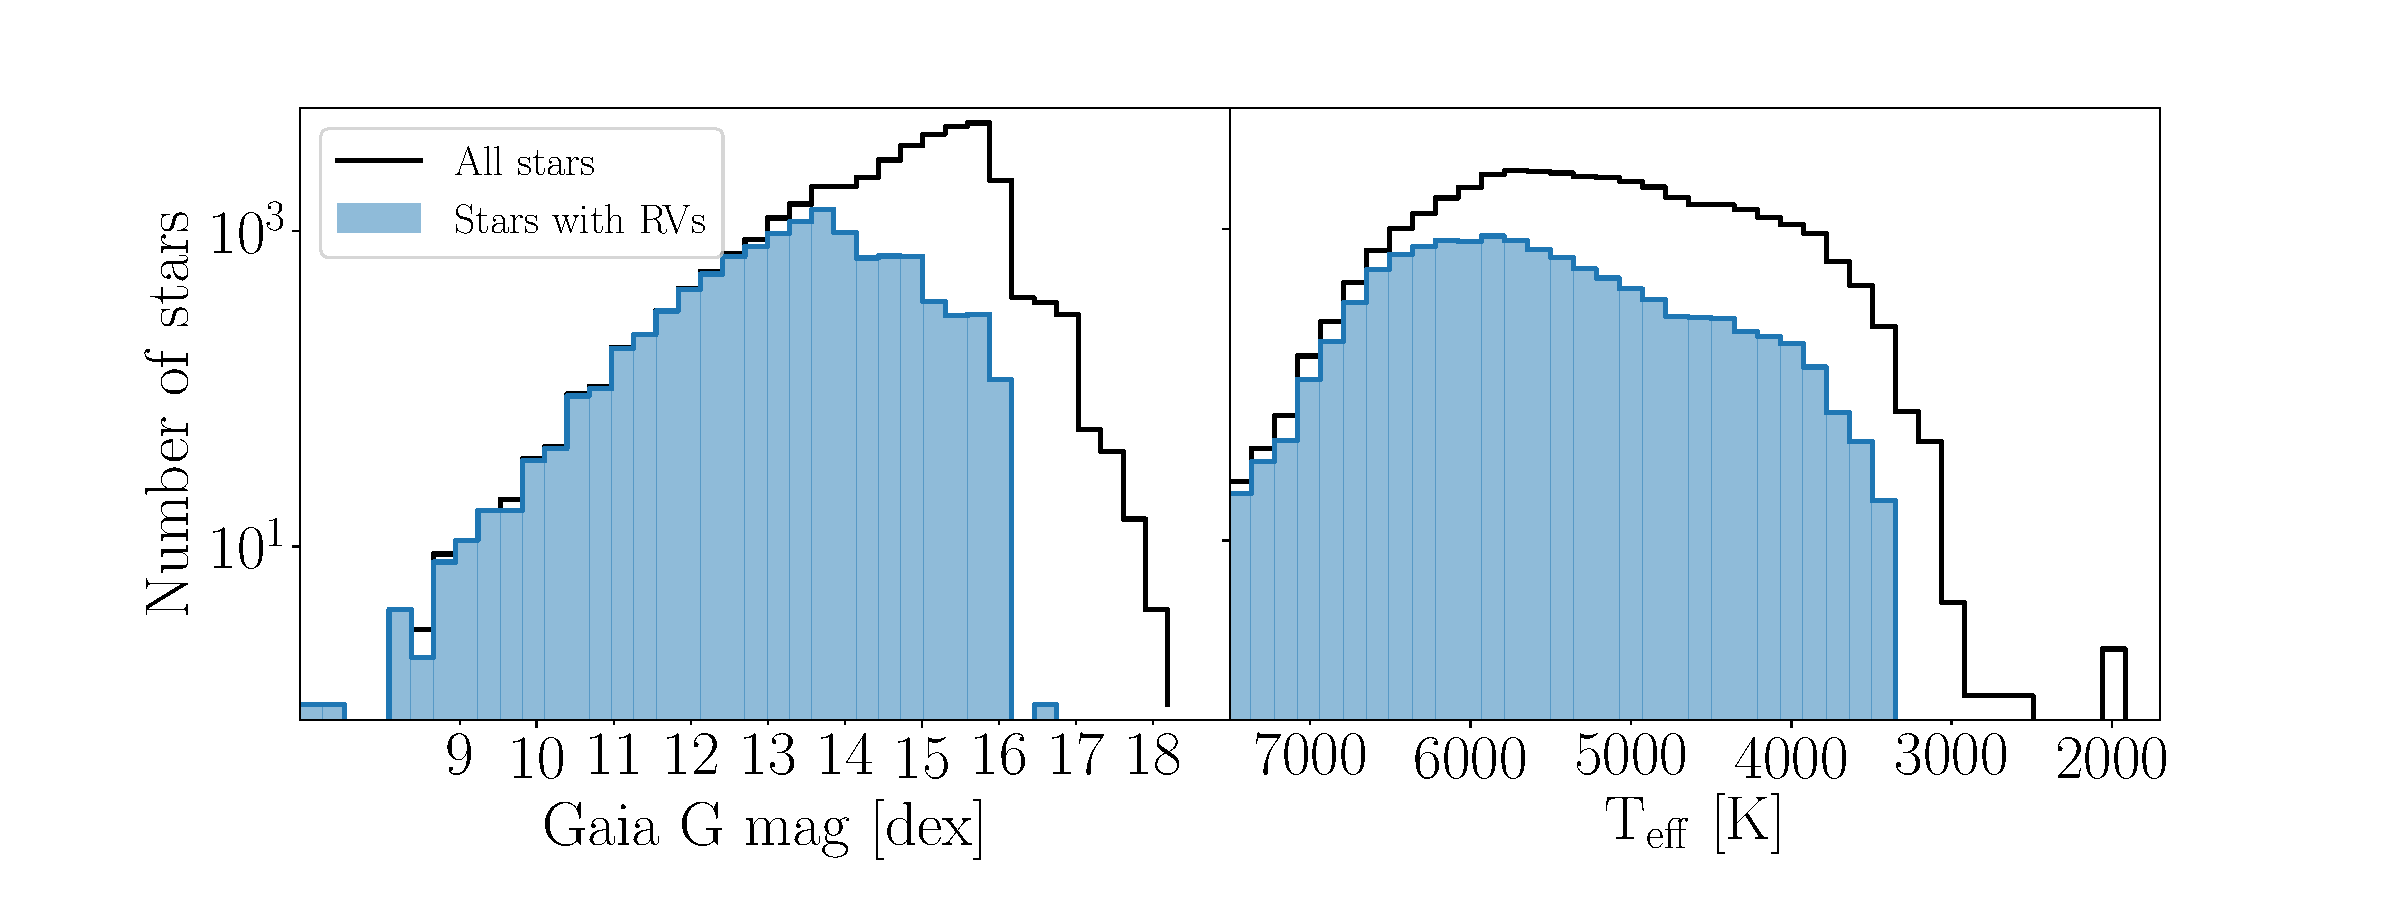
\includegraphics[width=1\textwidth]{rv_histogram}
\label{fig:rv_histogram}
\end{figure}
Given that rotational evolution is particularly poorly understood for M
dwarfs, the cool stars with missing RVs are arguably the most interesting.
To fill-in the low-temperature regime, we marginalized over missing RV
measurements to infer velocities for stars without RVs.
% \begin{figure}[ht!]
% \caption{
% Vertical velocity dispersion as a function of rotation period and effective
%     temperature for \kepler\ stars with measured rotation periods.
% Colored points show stars with RV measurements from \gaia\ or \lamost, with
%     their color indicating their velocity dispersion.
% Faint grey points show the combined \mct\ and \citet{santos2019} samples,
%     including stars without RV measurements.
% The coolest stars in this sample do not have RVs because they are faint.
% }
%   \centering 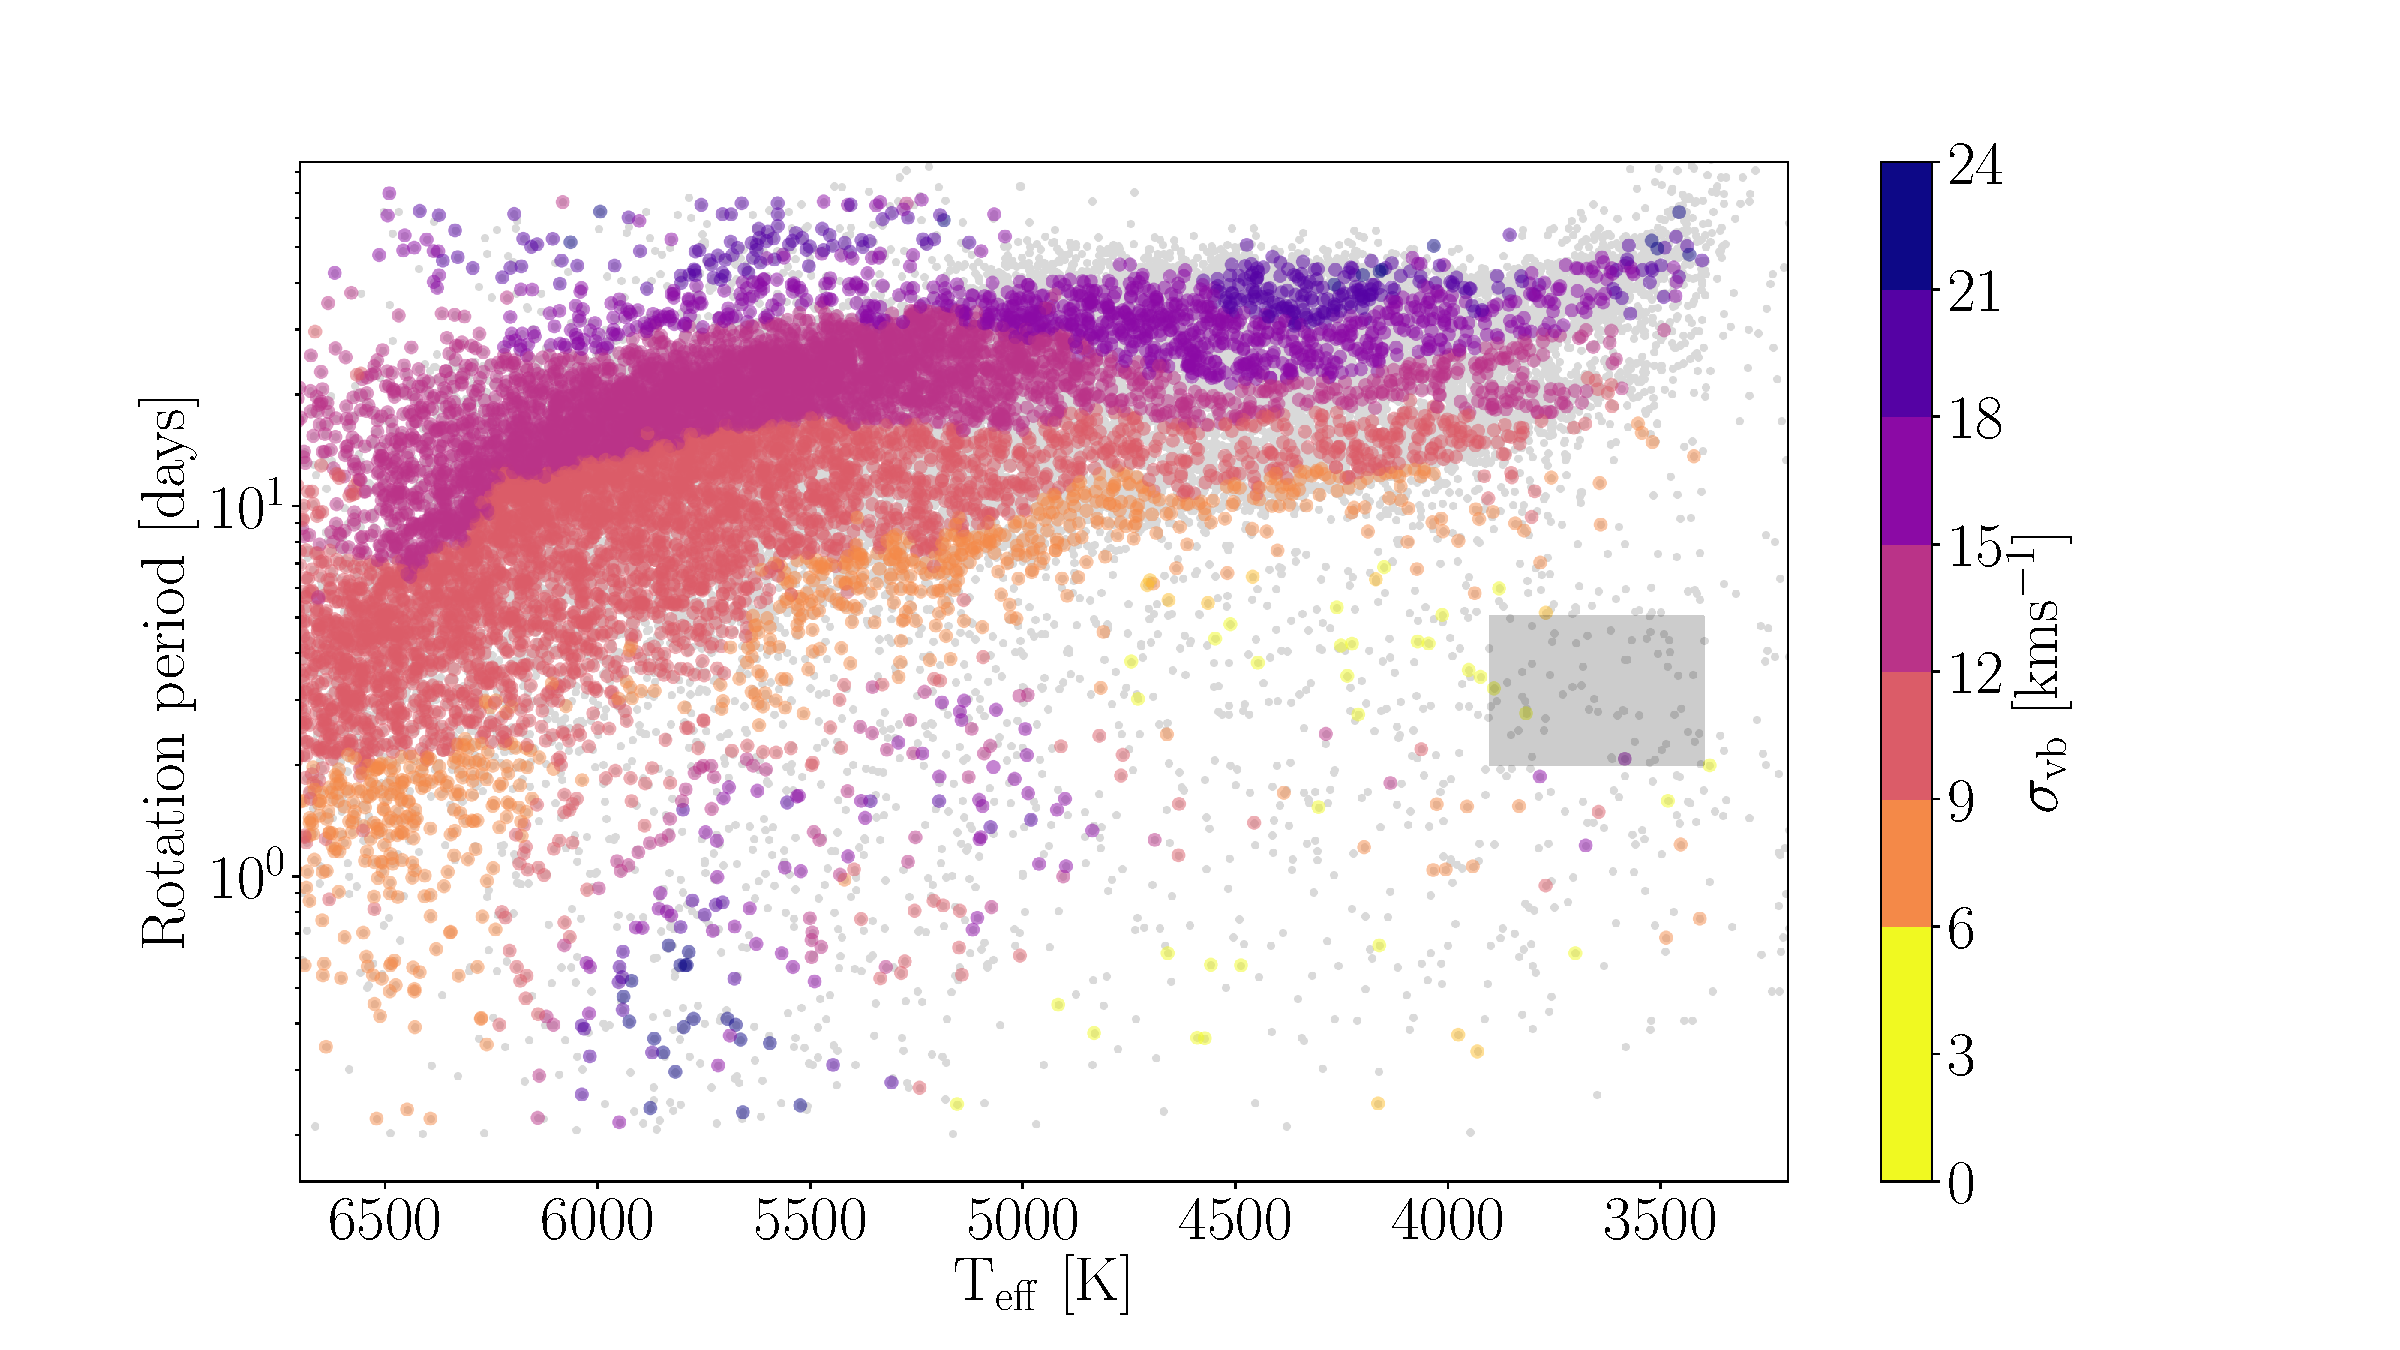
\includegraphics[width=1\textwidth]{existing_rvs}
% \label{fig:existing_rvs}
% \end{figure}

\subsection{Inferring 3D velocities (marginalizing over missing RV
measurements)}
\label{sec:inference}

% Three-dimensional velocities in galactocentric coordinates: \vx, \vy, and \vz\
% can only be directly computed via a transformation from 3D velocities in
% another coordinate system, like the equatorial coordinates provided by \gaia:
% \mura, \mudec, and RV.
% For stars with no measured RV in \gaia\ DR2, \vx, vy, and \vz\ can still be
% inferred from positions and proper motions alone, by marginalizing over
% missing RV measurements.
For each star in our sample, we inferred \vx, \vy, and \vz\ from the 3D
positions (right ascension, \ra, declination, \dec, and parallax, \parallax)
and 2D proper motions (\mura and \mudec) provided in the \gaia\ DR2 catalog
\citep{brown2011}.
We also simultaneously inferred distance, (instead of using inverse-parallax),
to model velocities \citep[see \eg][]{bailer-jones2015, bailer-jones2018}.

Using Bayes rule, the posterior probability of the parameters given the data
can be written:
\begin{equation}
    p({\bf v_{xyz}}, D | \mu_{\alpha}, \mu_{\delta}, \alpha, \delta, \pi) =
    p(\mu_{\alpha}, \mu_{\delta}, \alpha, \delta, \pi | {\bf v_{xyz}}, D)
    p({\bf v_{xyz}}) p(D),
\end{equation}
where $D$ is distance and ${\bf v_{xyz}}$ is the 3D vector of velocities.
Our model predicted observable data from model parameters,
\ie\ it converted \vx, \vy\, \vz\ and $D$ to \pmra, \pmdec\ and \parallax.
In the first step of the model, cartesian coordinates, \x, \y, and \z\, were
calculated from \ra\ and \dec\ measurements and $D$ ($1/\pi$) for each star,
by applying a series of matrix rotations, and a translation to account for the
Solar position.
The cartesian Galactocentric velocity parameters, \vx, \vy, and \vz, were then
converted to equatorial coordinates \pmra\ and \pmdec\ via another rotation.

As mentioned previously, the specific positioning of the \kepler\ field (at
low Galactic latitude) allows \vz\ to be well-constrained from proper motion
measurements alone.
This also happens to be the case for \vx, because the direction of the
\kepler\ field is almost aligned with the \y-axis of the Galactocentric
coordinate system and is almost perpendicular to both the \x\ and \z-axes (see
figure \ref{fig:kepler_field}).
For this reason, the \y-direction is similar to the radial direction for
observers near the Sun, so \vy\ will be poorly constrained without an RV
measurement for \kepler\ stars.
On the other hand, \vx\ and \vz\ are almost perpendicular to the radial
direction and can be precisely inferred with proper motions alone.
\begin{figure}[ht!]
\caption{
\x, \y\ and \z\ positions of stars observed by \kepler, showing the
    orientation of the \kepler\ field.
The direction of the field is almost aligned with the \y-axis and almost
    perpendicular to the \x\ and \z-axes, which is why \vx\ and \vz\ can be
    tightly constrained for stars without RVs, but \vy\ cannot.
}
  \centering
    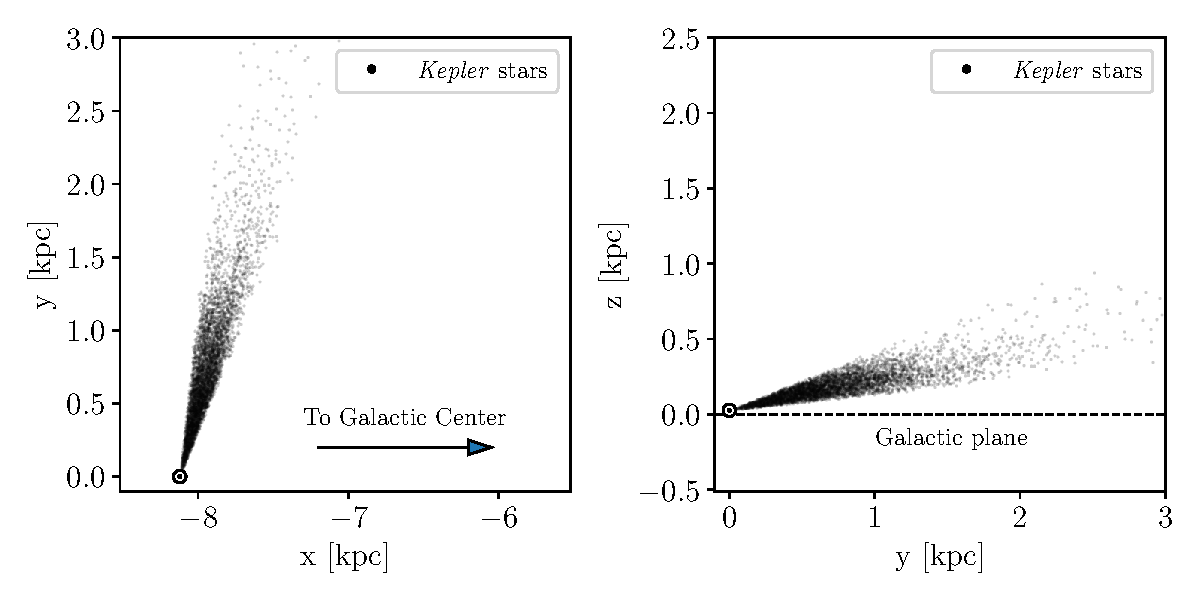
\includegraphics[width=.7\textwidth]{kepler_field}
\label{fig:kepler_field}
\end{figure}

\subsection{The prior}
\label{sec:prior}

The prior distribution over distance and velocities was constructed from the
data.
We calculated the means and covariances of the \vx, \vy, \vz\ and $\ln(D)$
distributions of stars {\it with measured RVs} and then used these means and
covariances to construct a multivariate Gaussian prior over the parameters for
stars {\it without} RVs.
Velocity outliers greater than 3-$\sigma$ were removed before calculating the
means and covariances of the distributions.
The 2-dimensional log-distance and velocity distributions are displayed in
figure \ref{fig:prior_distributions_2D}, with 2-$\sigma$ contours shown in
blue.
\begin{figure}[ht!]
\caption{
The 2D velocity and distance distributions for stars with RV measurements,
    used to construct a multivariate Gaussian prior over velocity and
    distance parameters for stars {\it without} RVs.
2-$\sigma$ contours are shown in blue.
}
  \centering
    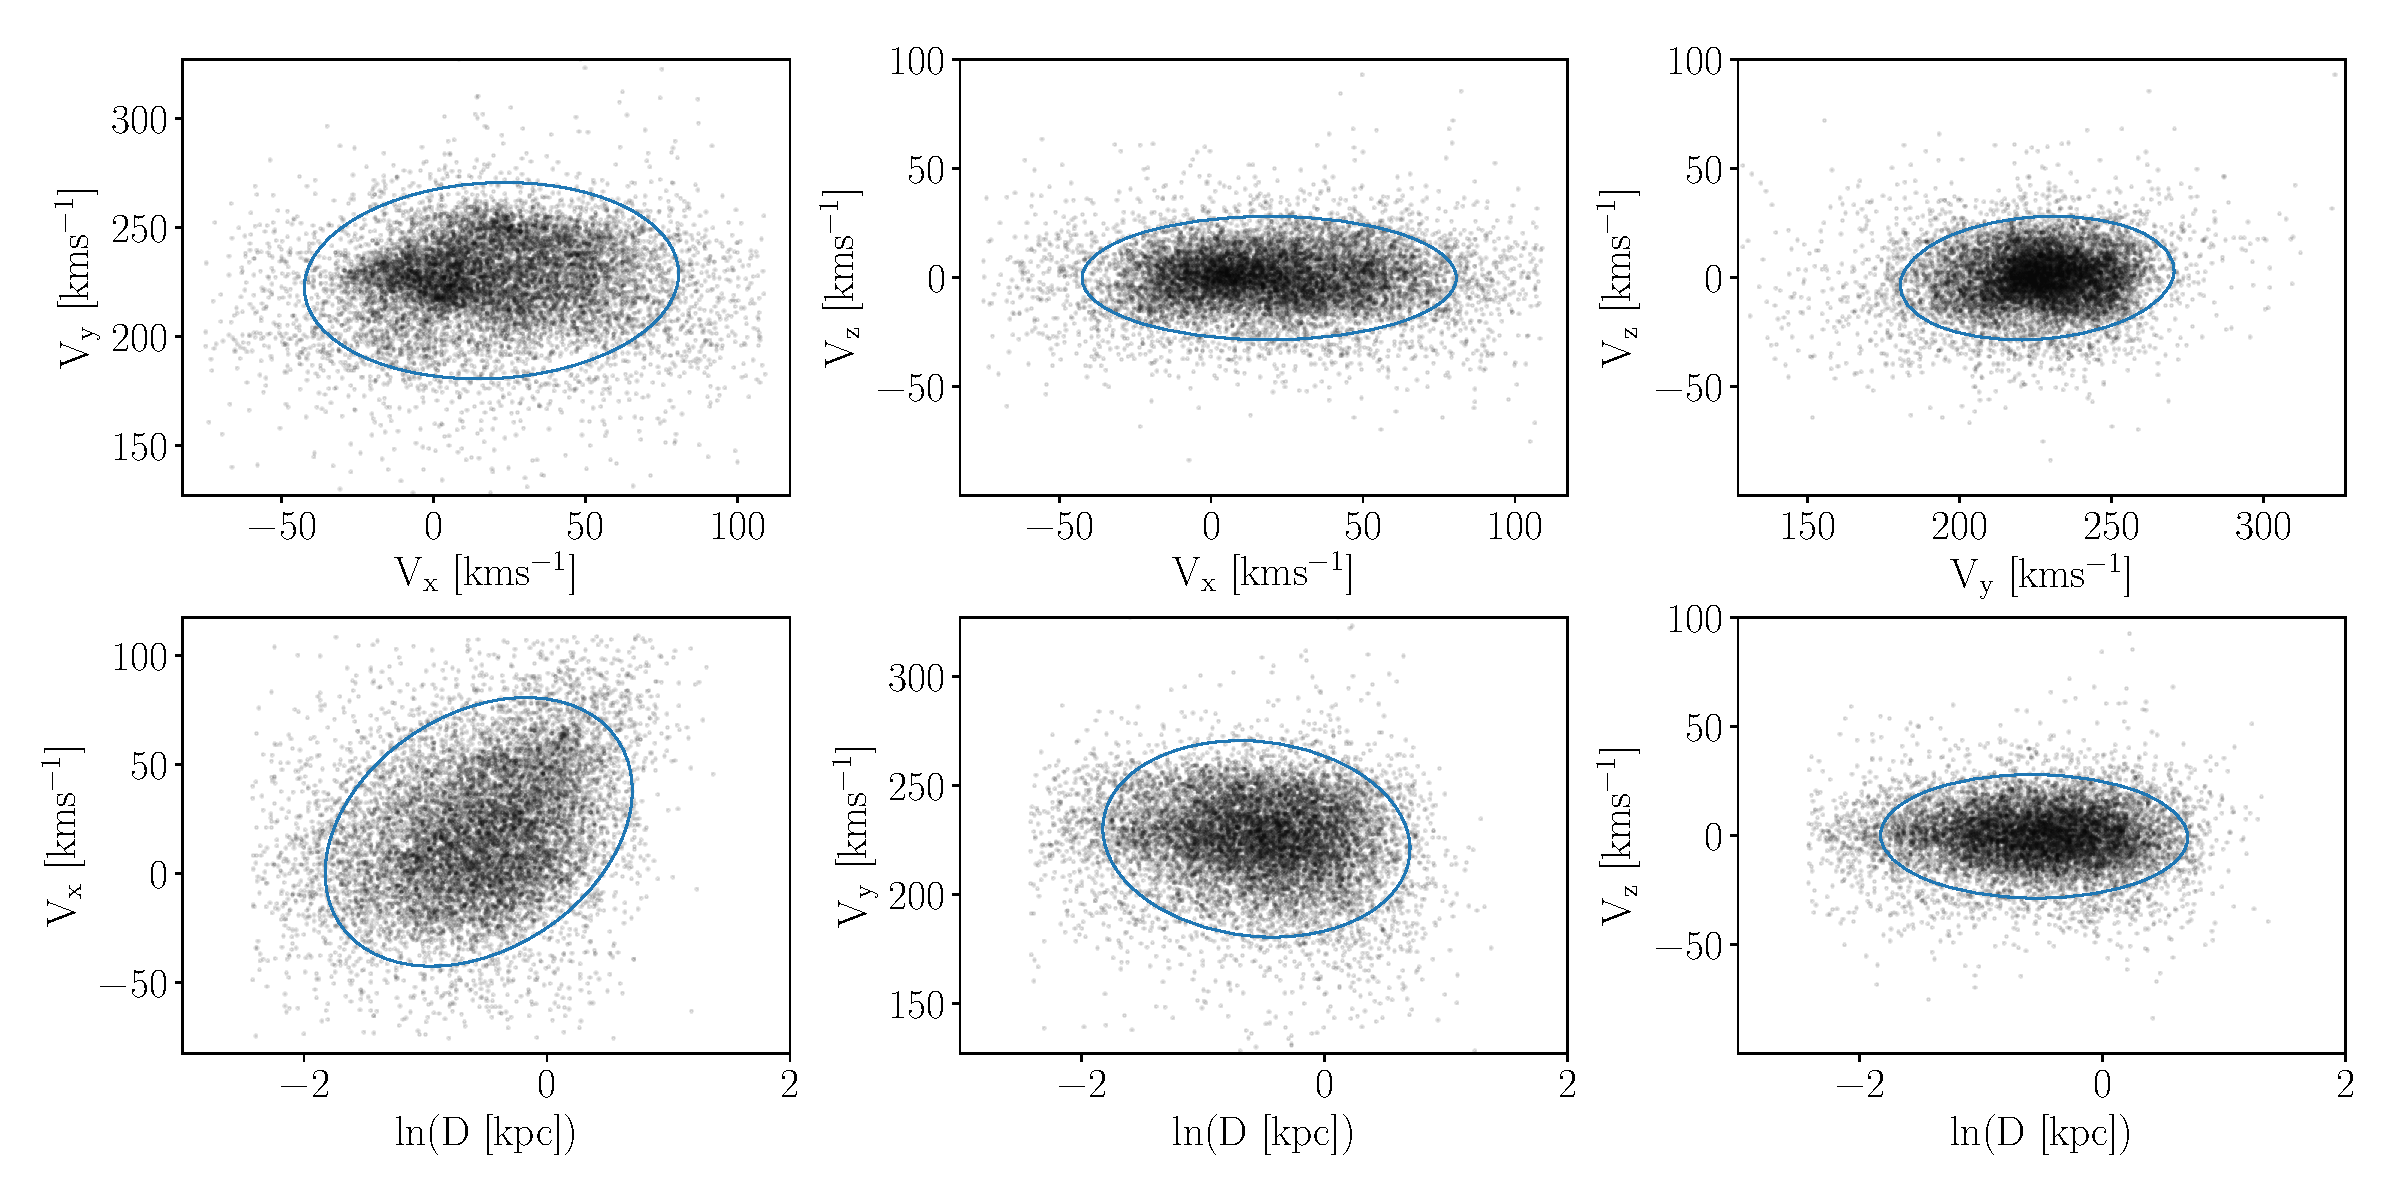
\includegraphics[width=1\textwidth]{prior_distributions_2D}
\label{fig:prior_distributions_2D}
\end{figure}

Our goal was to infer the velocities of stars {\it without} RV measurements
using a prior calculated from stars {\it with} RV measurements.
However, stars with and without RVs are likely to be different populations,
with parameters that depend on the \gaia\ and \lamost\ selection functions.
In particular, stars without RV measurements are more likely to be fainter and
cooler (\eg\ figure \ref{fig:rv_histogram}).
Lower-mass stars are, on average, older, and have larger velocity dispersions.
So a prior based on the velocity distributions of stars with RVs will not
necessarily reflect the velocities of those without.
However, given that \vx\ and \vz\ are likely to be relatively insensitive to
the prior as they are mostly informed by proper motion measurements, the prior
may impact our final vertical velocity dispersion measurements very little
(and this is the real quantity we care about).

We tested the effect of the prior on the velocities we inferred.
Three priors were tested: one calculated from the velocity distributions of
the brightest half of the RV sample (\gaia\ $G$-band apparent magnitude $<$
13.9), one from the faintest half ($G$ $>$ 13.9), and one from all stars with
RVs.
We inferred the velocities of 3000 stars chosen at random from the
\gaia-\lamost\ RV sample using each of these three priors and compared the
inferred velocity distributions.
If the inferred velocities were highly prior-dependent, these distributions
would look very different.
The results of this test are shown in figure \ref{fig:prior_comparison}.
From left to right, the three panels show the distributions of inferred \vx,
\vz, and \vy.
The blue dashed line shows a kernel density estimate, representing the
distributions of velocities inferred using a prior calculated from the faint
half of the RV sample.
Similarly, the solid orange line shows the same thing for a prior calculated
from the bright half of the RV sample, and the solid black line shows the
results of a prior calculated from all stars with measured RVs.
The \vx\ and \vz\ distributions are similar, regardless of the prior choice,
because velocities in the \x\ and \z-directions are not strongly prior
dependent: they are tightly constrained with proper motion measurements.
However, the distribution of inferred \vy\ velocities does depend on the
prior.
This is because the \y-direction is close to the radial direction for \kepler\
stars (figure \ref{fig:kepler_field}), and \vy\ cannot be tightly constrained
without an RV measurement.
It is therefore highly dependent on the prior.
\begin{figure}[ht!]
\caption{
    }
  \centering
    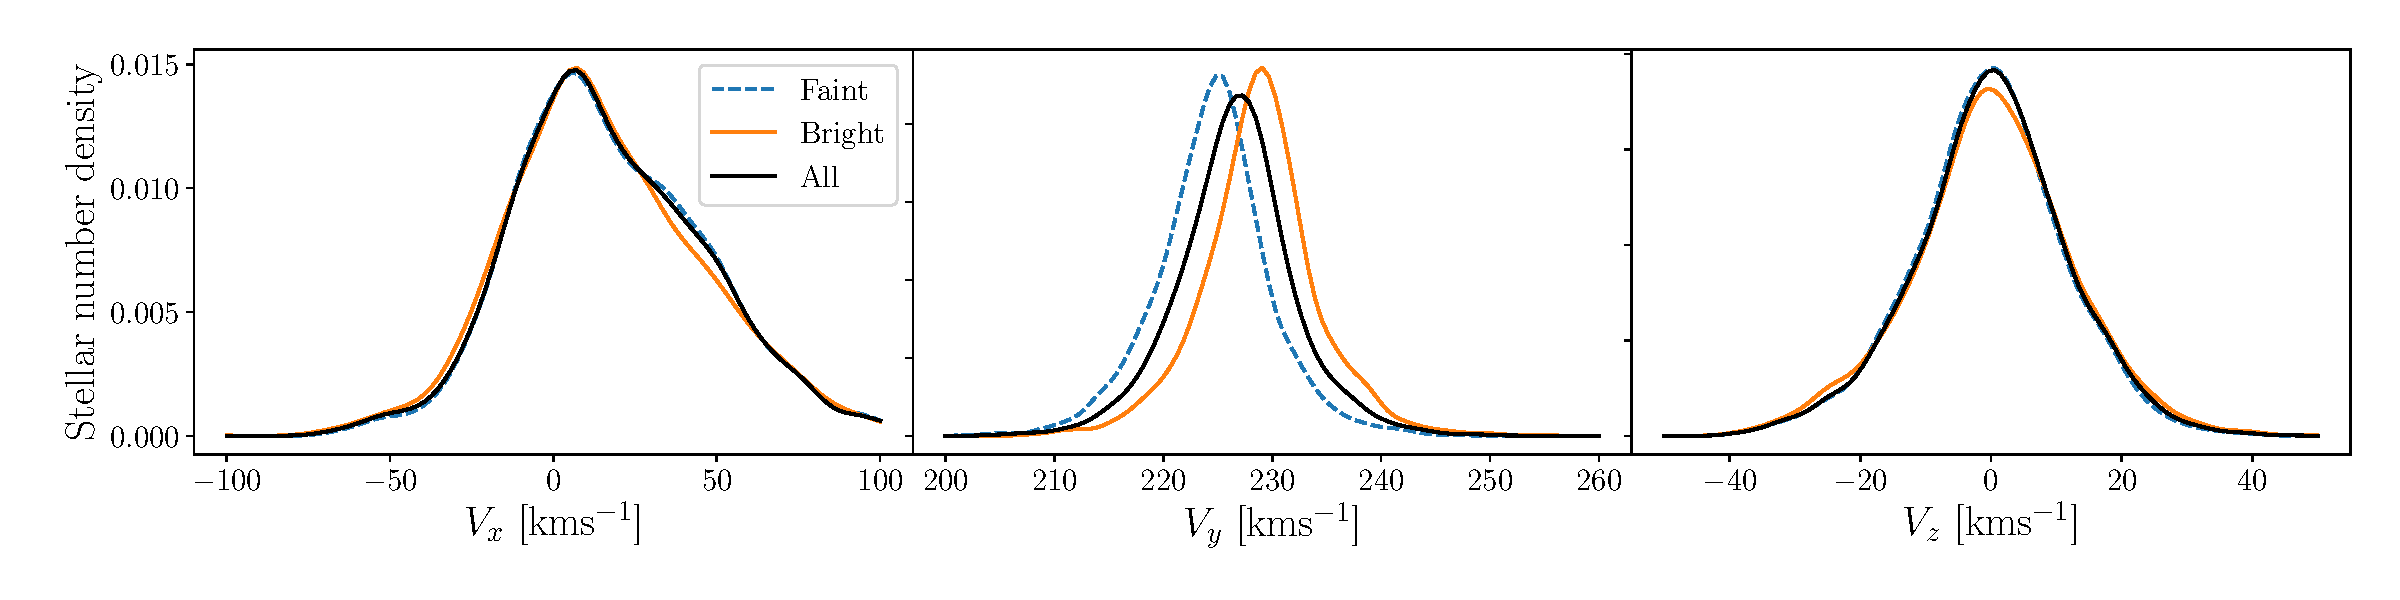
\includegraphics[width=1\textwidth]{prior_comparison}
\label{fig:prior_comparison}
\end{figure}

% The mean values of the \vy\ distributions differ by around 4 \kms.
% Fainter stars have smaller y-velocities than brighter stars because they are,
% on average, further from the Sun

Although this test was performed on stars with RV measurements, which are
brighter overall than the sample of stars without RVs (\eg\ figure
\ref{fig:rv_histogram}), figure \ref{fig:prior_comparison} nevertheless shows
that \vx\ and \vz\ are not strongly prior-dependent.
In this work we are only concerned with \vz, as we only use {\it vertical}
velocity dispersion as an age indicator.
The difference in the dispersions of \vz\ velocities, calculated with the
three different priors tested above was smaller than 0.5 \kms.
We therefore conclude that vertical velocity dispersion is relatively
insensitive to prior choice, and we adopt a prior calculated from the
distributions of all stars with RV measurements.

% \begin{figure}[ht!]
% \caption{
%     }
%   \centering
%     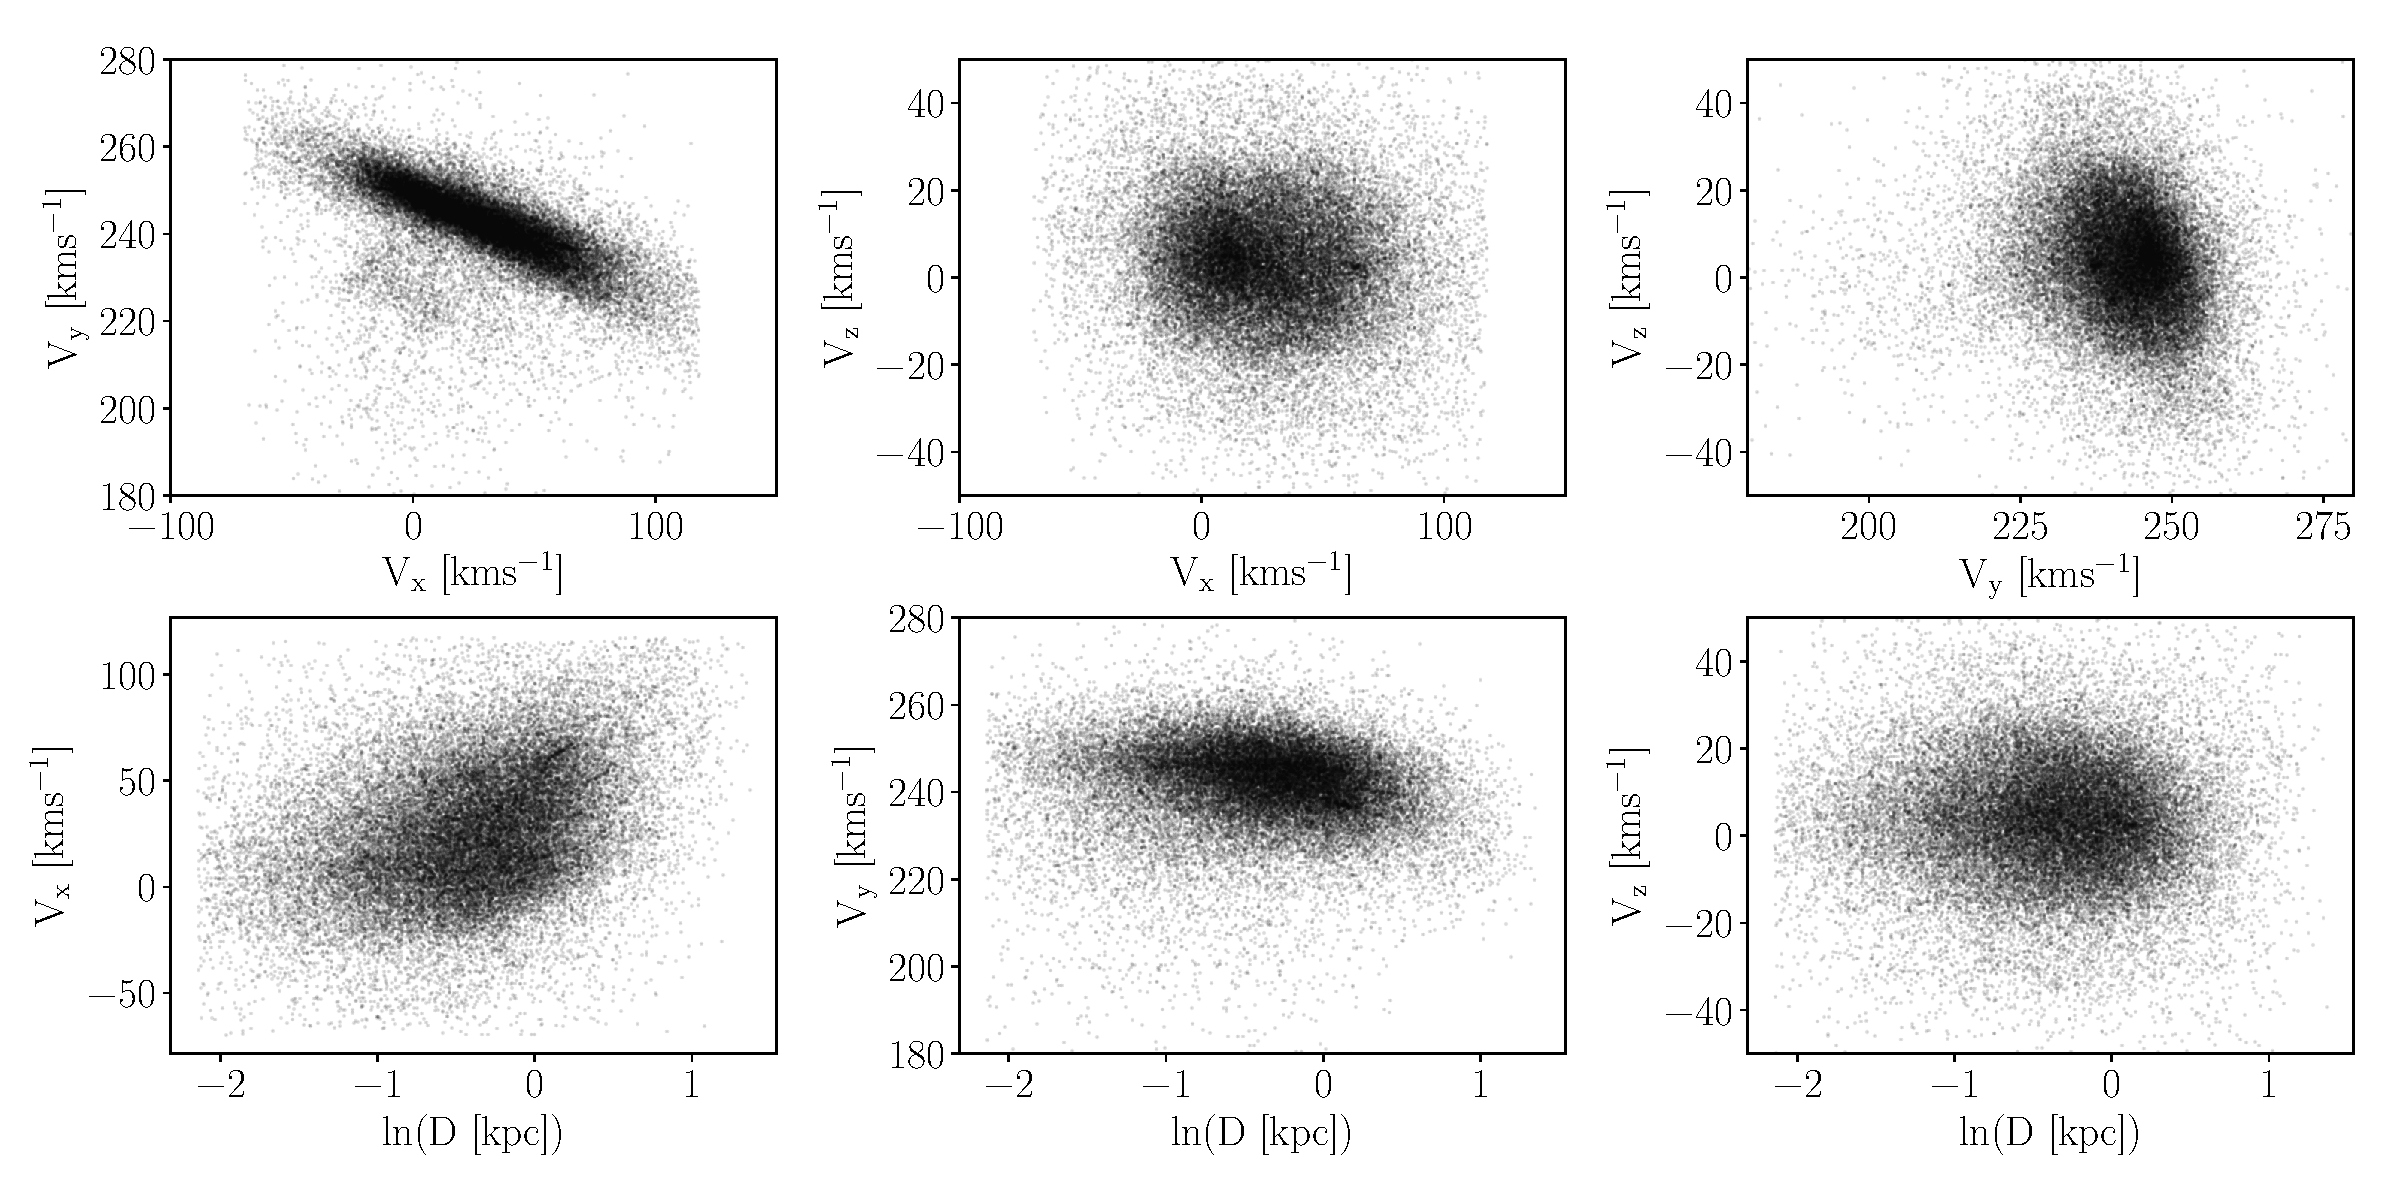
\includegraphics[width=1\textwidth]{prior_distributions}
% \label{fig:prior_distributions}
% \end{figure}

\subsection{Inferred velocities}

For each star in the \kepler\ field, we explored the posteriors of these four
parameters using the {\it PyMC3} No U-Turn Sampler (NUTS) algorithm, and the
{\tt exoplanet} \python\ library \racomment{(citations)}.
We tuned the {\it PyMC3} sampler for 1500 steps, with a target acceptance
fraction of 0.9, then ran four chains of 1000 steps for a total of 4000 steps.
Using PyMC3 made the inference procedure exceptionally fast -- taking just a
few seconds per star on a laptop.

To validate this method, we inferred velocities for stars in our sample with
measured RVs and compared those inferred values with velocities calculated
directly from 6D position, proper motion, and RV measurements.
Figure \ref{fig:residuals} shows the \vx, \vy\ and \vz\ velocities we
inferred, for 3000 stars chosen at random, compared with those calculated from
measured RVs.
\begin{figure}[ht!]
\caption{Vertical velocities calculated with full 6D information vs vertical
    velocities inferred without RV, for 3000 \mct\ stars with \gaia\ RV
    measurements.}
  \centering
    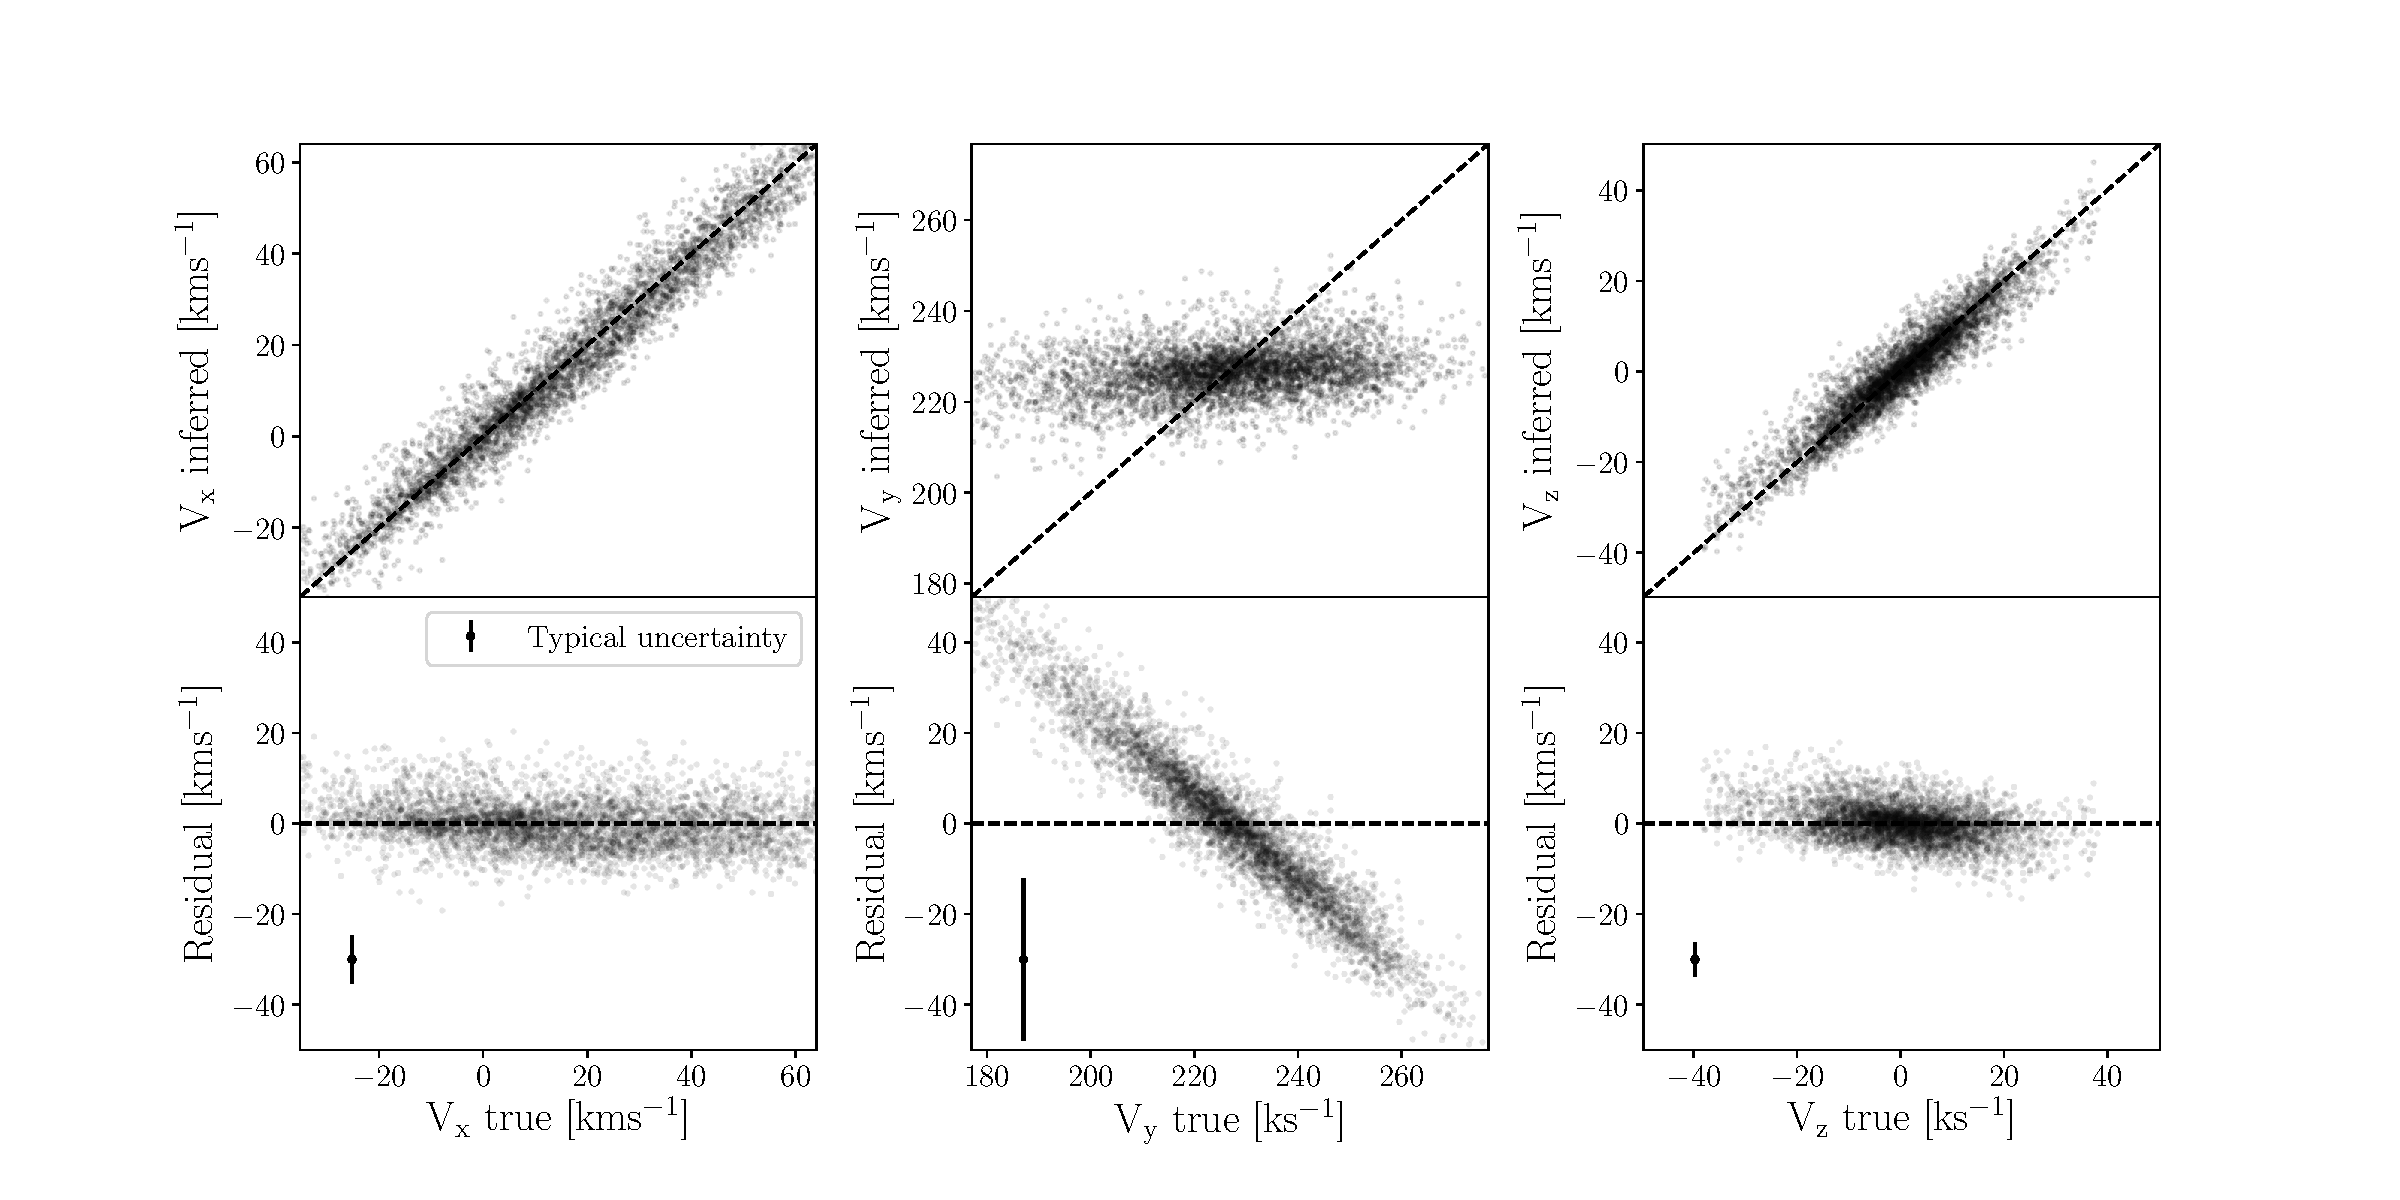
\includegraphics[width=1\textwidth]{residuals}
\label{fig:residuals}
\end{figure}

The three velocity components, \vx, \vy\ and \vz\ were recovered with
differing levels of precision: \vx\ and \vz\ are inferred more precisely than
\vy.
This is because of the orientation of the \kepler\ field, shown in figure
\ref{fig:kepler_field}.
\racomment{Slight inaccuracies seen in the residual panels for \vx\ and \vz\
are caused by ....
Quote some summary statistics.}

